% Slides for 2025-08-05
% To create a slide, use the following:
% \begin{frame}{TITLE}
%     BODY
% \end{frame}

% To create a slide with a bullet list, use the following:
% \begin{frame}{TITLE}
%     \begin{itemize}
%         \item ITEM 1
%         \item ITEM 2
%     \end{itemize}    
% \end{frame}

% To create a slide with numbered list, use the following:
% \begin{frame}{TITLE}
%     \begin{enumerate}
%         \item ITEM 1
%         \item ITEM 2
%     \end{enumerate}
% \end{frame}

% To create a slide with a graphic:
% 1. Add the graphic to this folder (named picture.png)
% 2. Use the following:
% \begin{frame}{TITLE}
%     \centering
%     \includegraphics[height=0.7\textheight,width=0.7\textwidth,keepaspectratio]{picture.png}
% \end{frame}

% To create a slide with two columns, use the following:
% \begin{frame}{TITLE}
%     \begin{columns}
%         \begin{column}{0.5\textwidth}
%             COLUMN 1 BODY
%         \end{column}
%         \begin{column}{0.5\textwidth}
%             COLUMN 2 BODY
%         \end{column}
%     \end{columns}
% \end{frame}

\begin{frame}{Collar Team Agenda}
    \begin{itemize}
        \item Full Integration (Ready \& Almost Ready)
        \item Power Studies
        \item Battery Calculator
        \item Piezoelectric Sensor
        \item Future of Acoustic Collar
    \end{itemize}
\end{frame}

\begin{frame}{Full Integration - Ready}
    \begin{columns}
        \begin{column}{0.45\textwidth}
            \begin{itemize}
                \item Microphone working and clocked properly (1.024MHz)
                \item SAI/DMA working and clock properly
                \item Cortex-M7 can fetch PCM data, convert to PDM, generate mel spec, and run inference
                \item Optional audio playback for debugging
            \end{itemize}
        \end{column}
        \begin{column}{0.55\textwidth}
            \begin{figure}
                \centering
                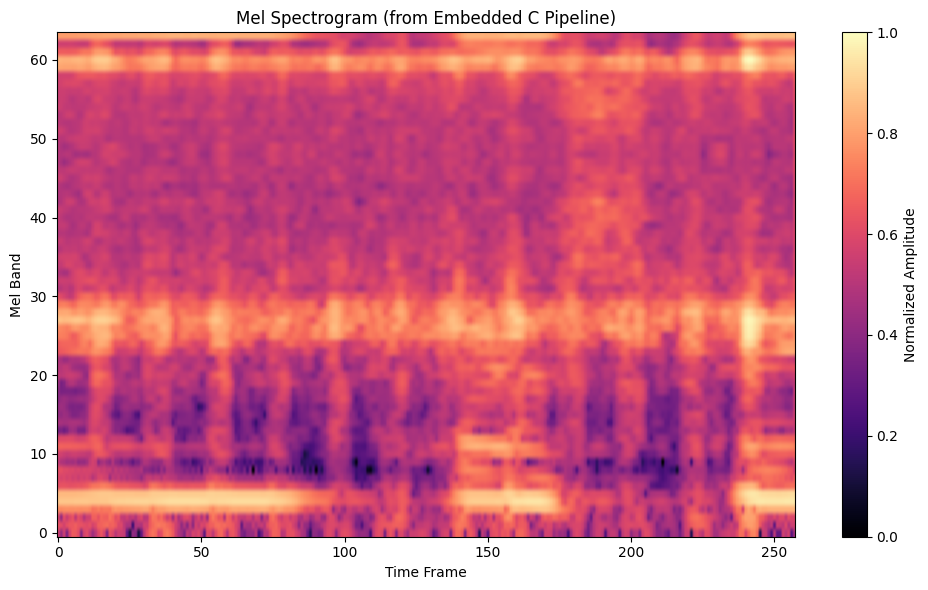
\includegraphics[height=1\textheight,width=1\textwidth,keepaspectratio]{images/mel_spec.png}
                \caption{Speech mel spectrogram}
            \end{figure}
        \end{column}
    \end{columns}
\end{frame}

\begin{frame}{Full Integration - Almost Ready}
    \begin{itemize}
        \item SAI clocks wrong → SD writes at wrong sampling rate 
        \item Wake-up trigger (piezo + op-amp)
        \item Write-up on issues encountered, design decisions, etc.
    \end{itemize}
\end{frame}

\begin{frame}{Power Studies}
    \begin{itemize}
        \item Sample
    \end{itemize}
\end{frame}

\begin{frame}{Battery Calculator}
    \begin{itemize}
        \item Sample
    \end{itemize}
\end{frame}

\begin{frame}{Piezoelectric Sensor}
    \begin{itemize}
        \item All images taken at back of neck, two layers of fabric
        \item Notice not only amplitude, but frequency
        \item Even with layers of separation, easy to isolate
        \item Sampled on a single piezo bought on Amazon for \$0.60
    \end{itemize}
    \hspace{10pt}
    \begin{figure}
        \centering
        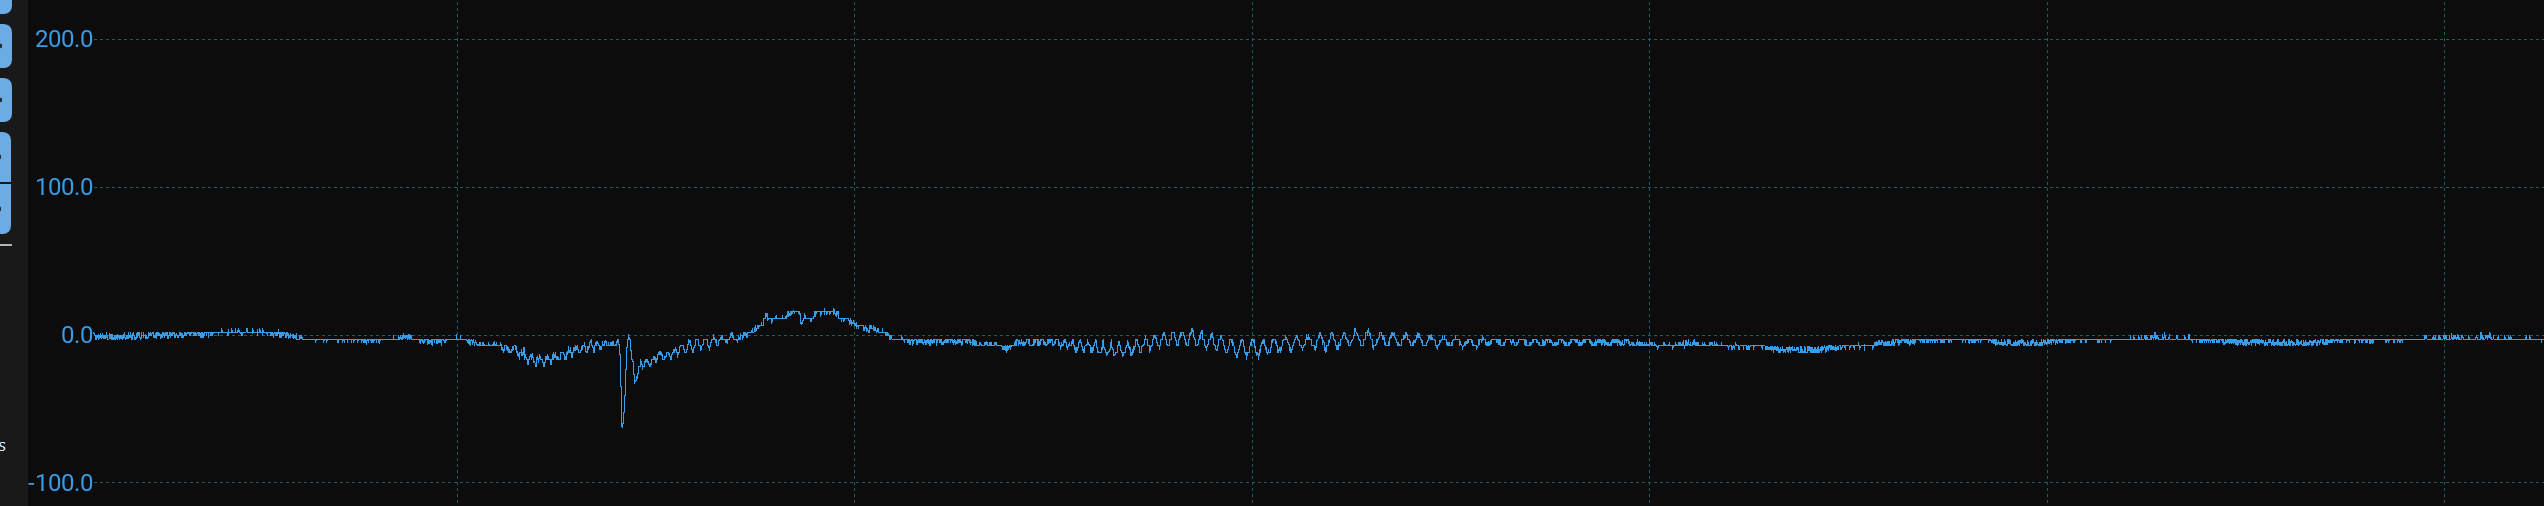
\includegraphics[height=0.8\textheight,width=1\textwidth,keepaspectratio]{images/piezo_hello_muffled.png}
        \caption{``Hello'' on the piezo}
    \end{figure}
\end{frame}

\begin{frame}{Piezoelectric Sensor (Contd.)}
    \begin{figure}
        \centering
        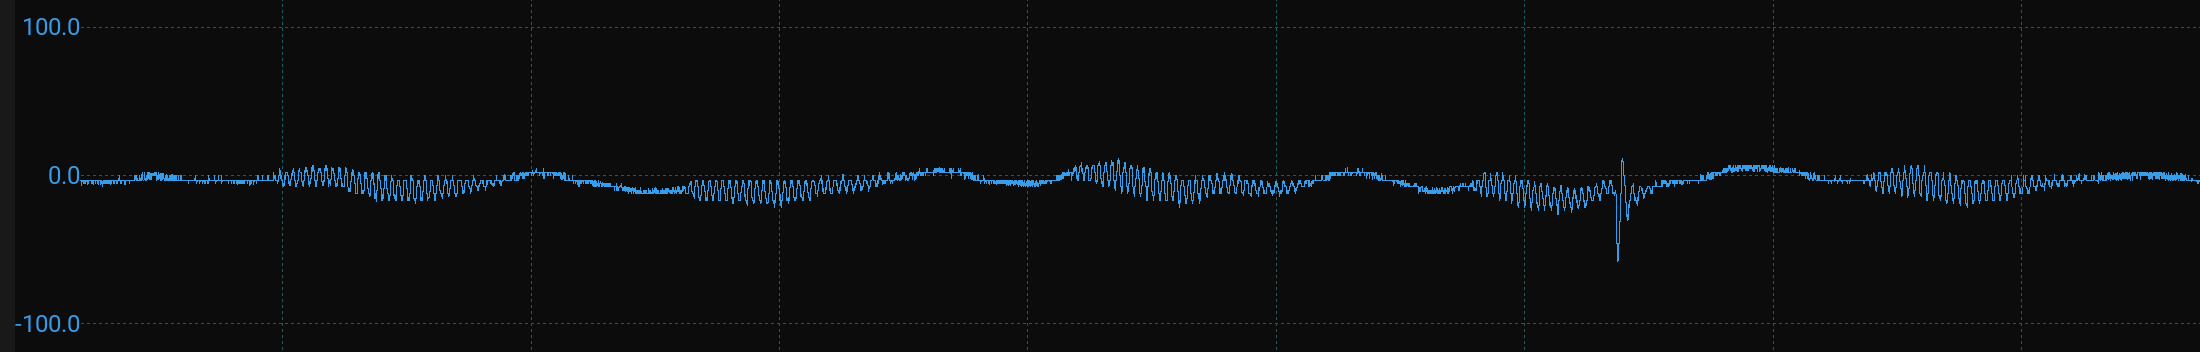
\includegraphics[height=0.5\textheight,width=0.9\textwidth,keepaspectratio]{images/piezo_chuffing_muffled.png}
        \caption{Chuffing recreated on the piezo}
    \end{figure}
    \begin{figure}
        \centering
        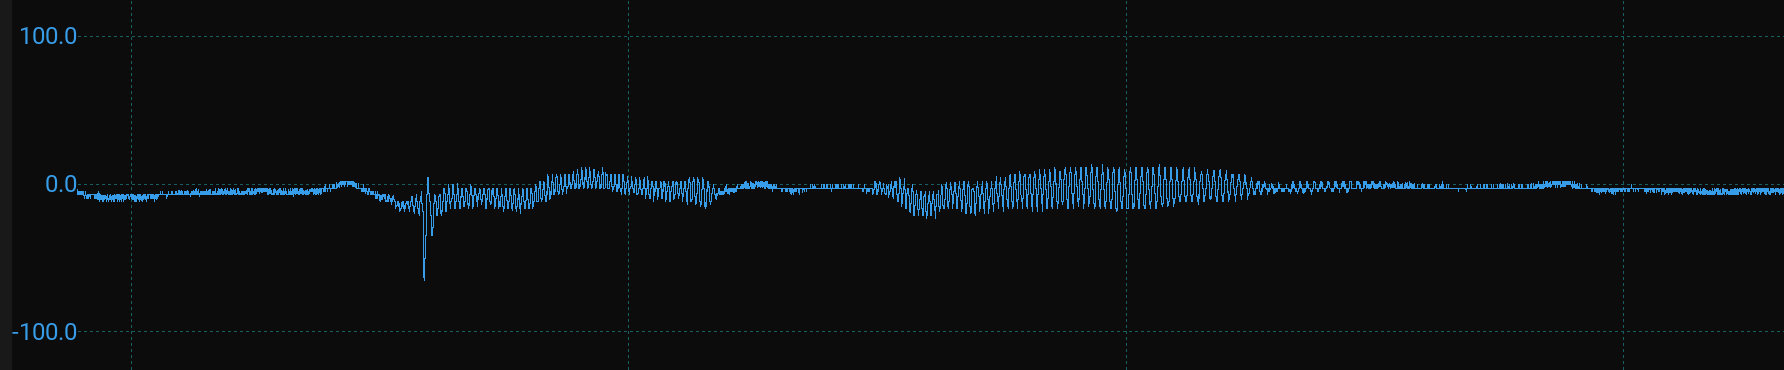
\includegraphics[height=0.5\textheight,width=0.8\textwidth,keepaspectratio]{images/piezo_roar_muffled.png}
        \caption{Roaring recreated on the piezo}
    \end{figure}
\end{frame}

\begin{frame}{Future of Acoustic Collar}
    \begin{itemize}
        \item Short-term
        \begin{itemize}
            \item Variant TinyML models for panda, polar bear, etc.
            \item RTC (Real-time Clock) labelling of samples
            \item Move to smaller board
        \end{itemize}
        \item Long-term
        \begin{itemize}
            \item LoRa Networking
        \end{itemize}
    \end{itemize}
\end{frame}

\begin{frame}{Autoencoders (Both Teams)}
    \begin{itemize}
        \item 
    \end{itemize}
    \begin{figure}
        \centering
        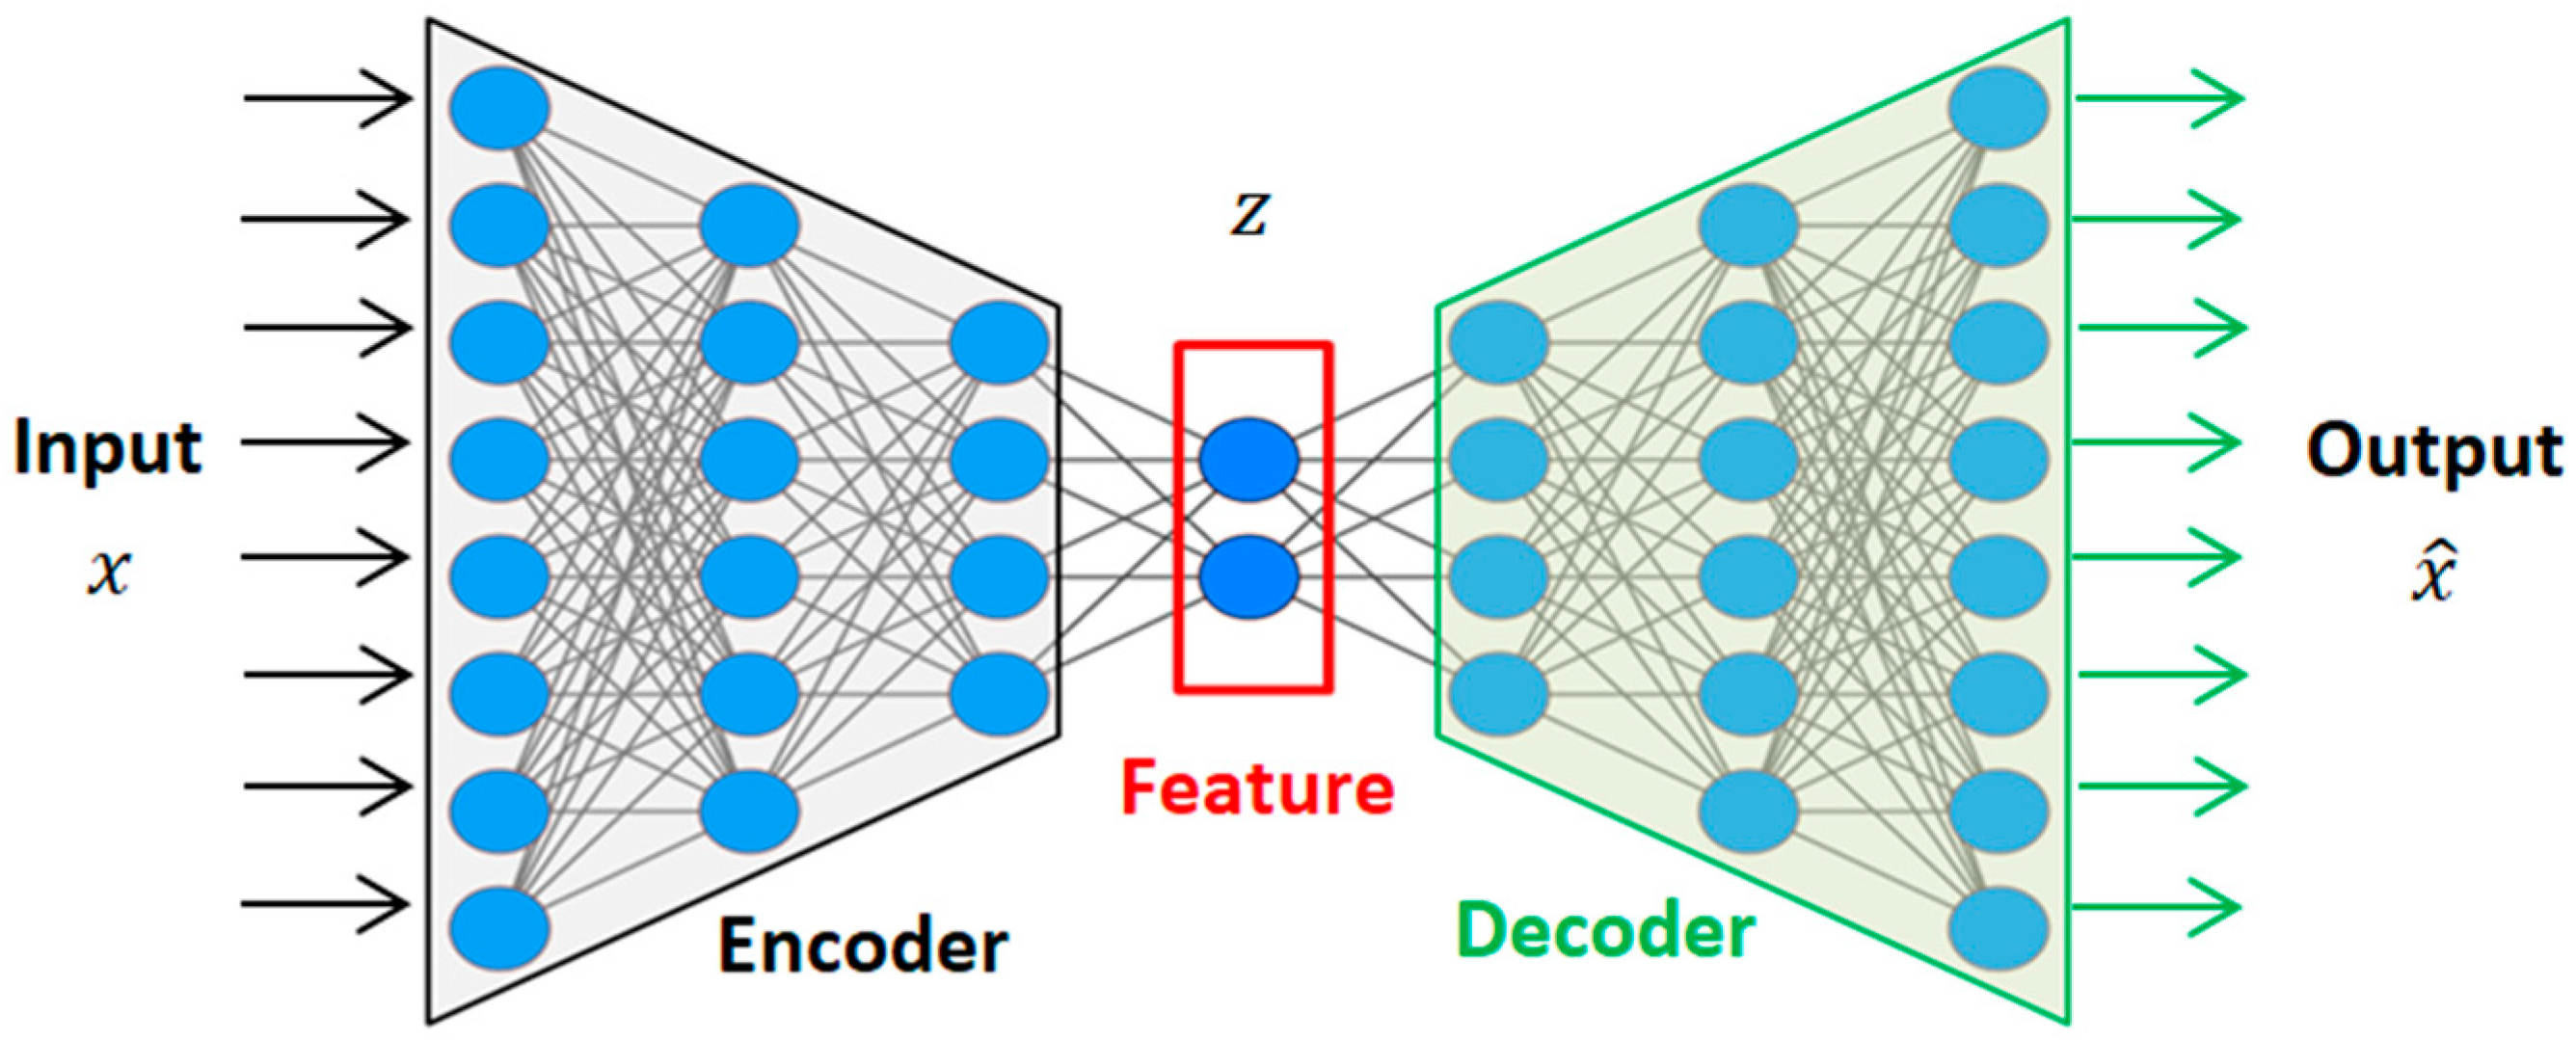
\includegraphics[height=0.7\textheight,width=0.7\textwidth,keepaspectratio]{images/autoencoder.png}
        \caption{Autoencoder architecture (Alaghbari et al., 2023)}
    \end{figure}
\end{frame}

\begin{frame}{ML Team Agenda}
    \begin{itemize}
        \item Desktop App
        \item Knowledge Graphs
        \item Regression
        \item Template Matching
        \item Binary Classifier
        \item Site Separation
        \item D3.JS Visualization
    \end{itemize}
\end{frame}

\begin{frame}{Desktop App}
    \begin{itemize}
        \item Sent to collaborators for feedback, scheduling meeting to address issues
    \end{itemize}
    \begin{figure}
        \centering
        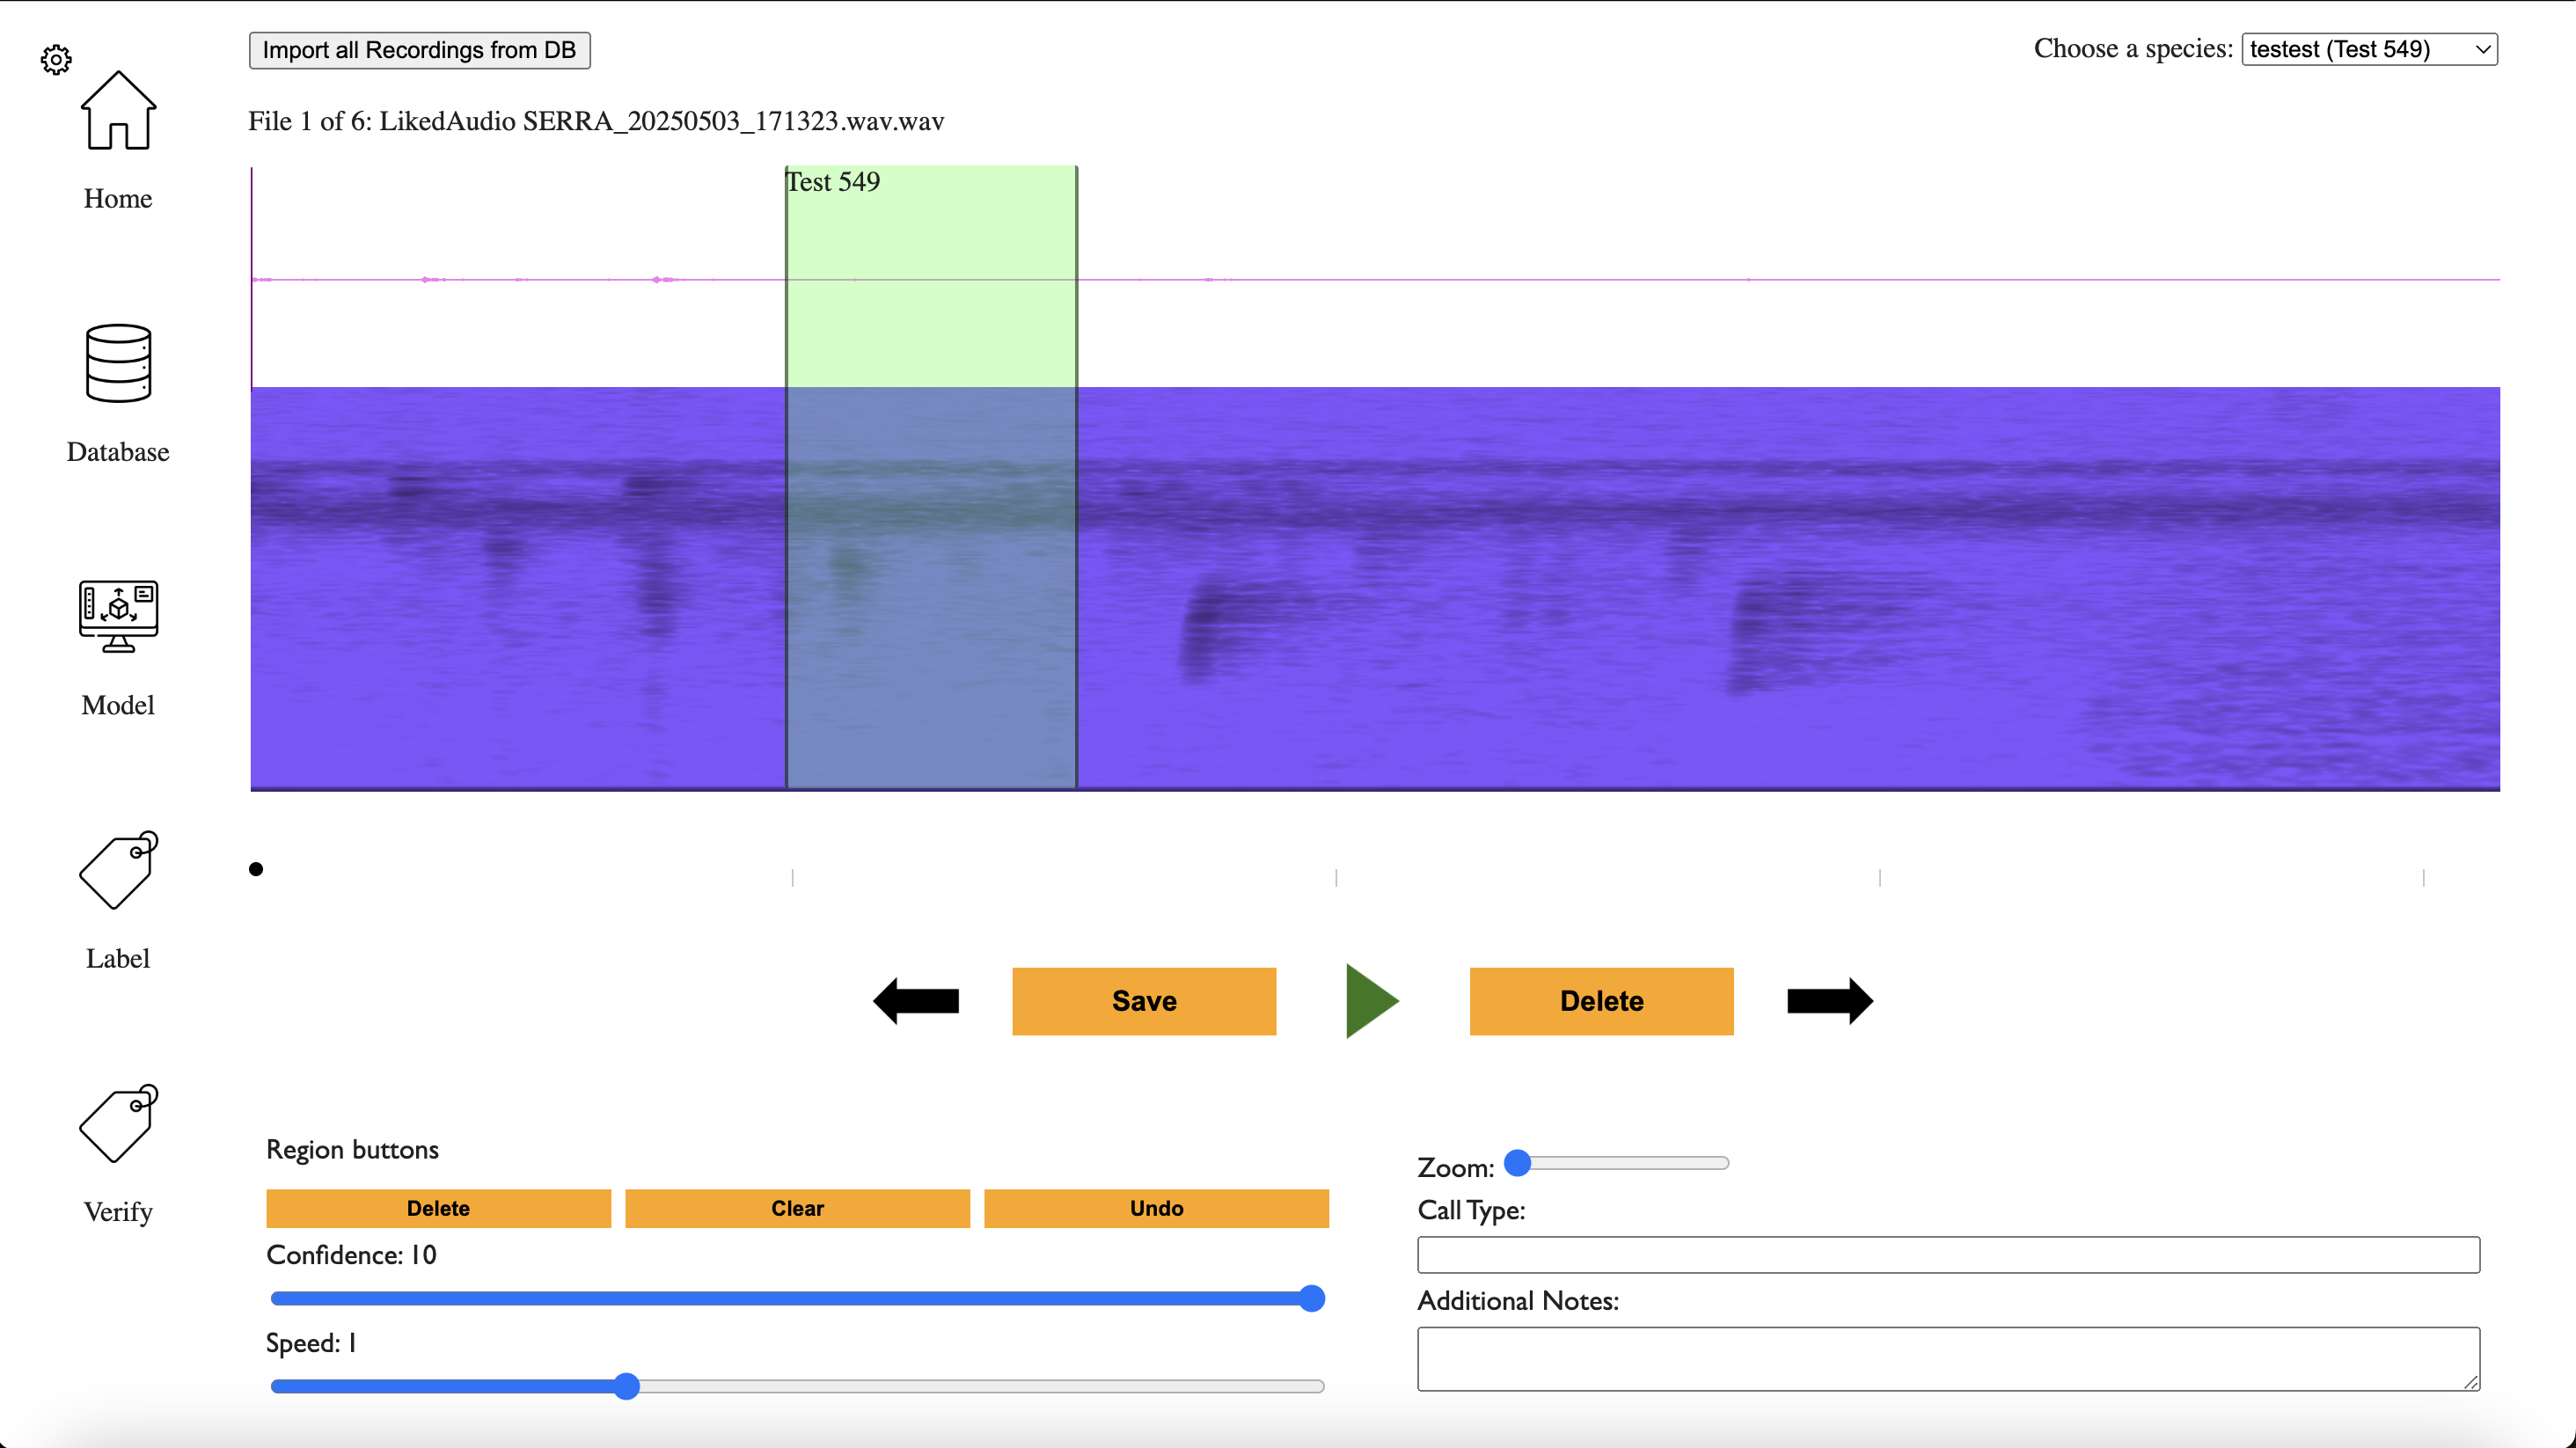
\includegraphics[height=0.7\textheight,width=0.7\textwidth,keepaspectratio]{images/desktop_app_1.png}
        \caption{Desktop App interface}
    \end{figure}
\end{frame}

\begin{frame}{Desktop App}
    \begin{figure}
        \centering
        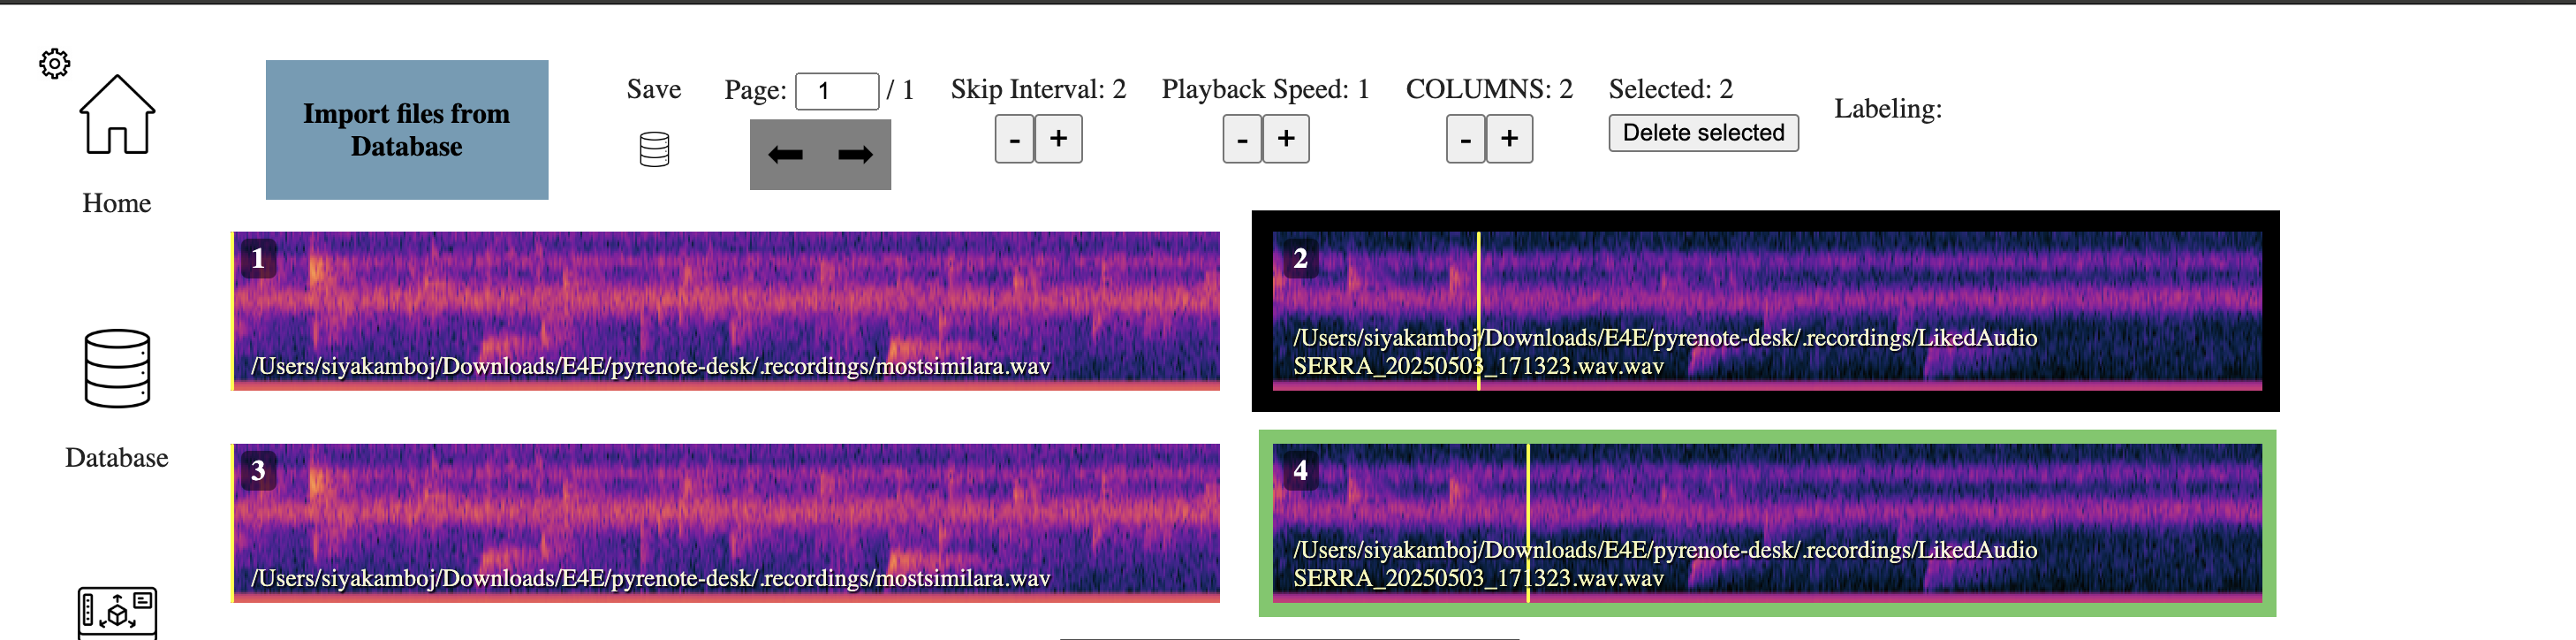
\includegraphics[height=1.0\textheight,width=1.0\textwidth,keepaspectratio]{images/desktop_app_2.png}
        \caption{Desktop App labeling interface}
    \end{figure}
\end{frame}

\begin{frame}{Knowledge Graphs - Input}
    \begin{columns}
        \begin{column}{0.3\textwidth}
            \begin{itemize}
                \item Inserted 2,231 of Paola's audio files
            \end{itemize}
        \end{column}
        \begin{column}{0.7\textwidth}
            \centering
            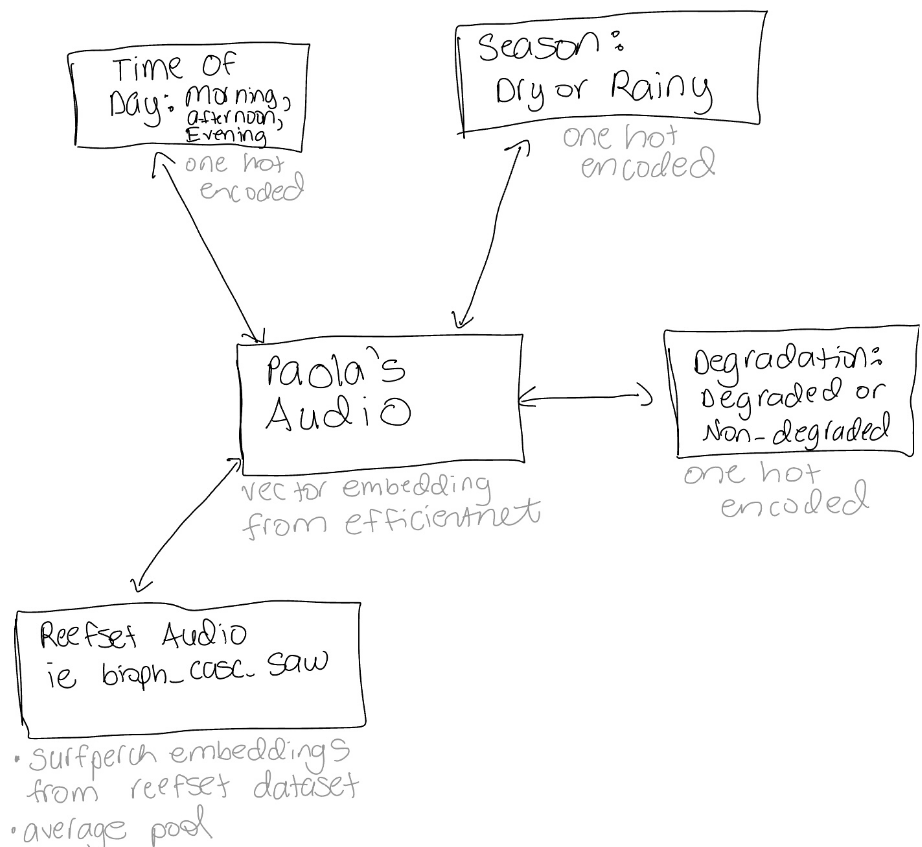
\includegraphics[height=0.8\textheight,width=0.8\textwidth,keepaspectratio]{images/knowledge_graph.png}
        \end{column}
    \end{columns}
\end{frame}

\begin{frame}{Knowledge Graphs - Results}
    \begin{columns}
        \begin{column}{0.7\textwidth}
            \centering
            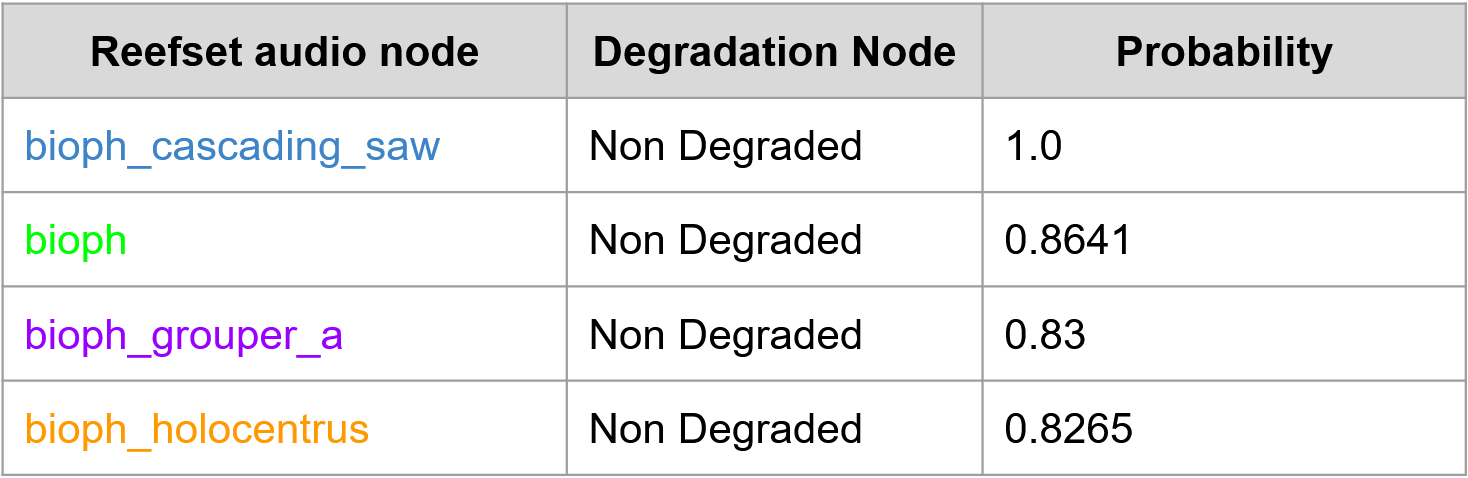
\includegraphics[height=1.0\textheight,width=1.0\textwidth,keepaspectratio]{images/knowledge_graph_table.png}
        \end{column}
        \begin{column}{0.3\textwidth}
            \centering
            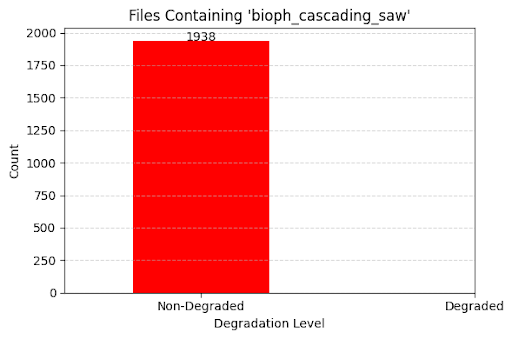
\includegraphics[height=1.0\textheight,width=1.0\textwidth,keepaspectratio]{images/knowledge_graph_results_1.png}
        \end{column}
    \end{columns}
    \hspace{1cm}
    \begin{columns}
        \begin{column}{0.33\textwidth}
            \centering
            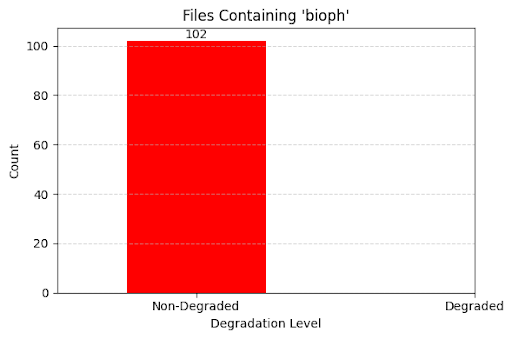
\includegraphics[height=1.0\textheight,width=1.0\textwidth,keepaspectratio]{images/knowledge_graph_results_2.png}
        \end{column}
        \begin{column}{0.33\textwidth}
            \centering
            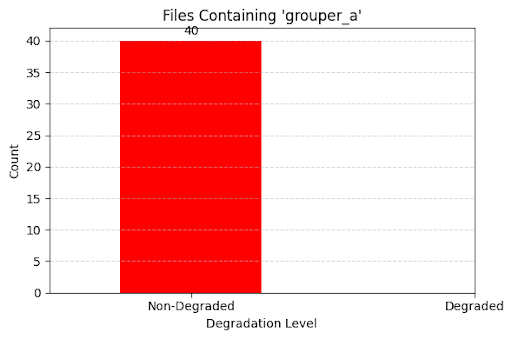
\includegraphics[height=1.0\textheight,width=1.0\textwidth,keepaspectratio]{images/knowledge_graph_results_3.png}
        \end{column}
        \begin{column}{0.33\textwidth}
            \centering
            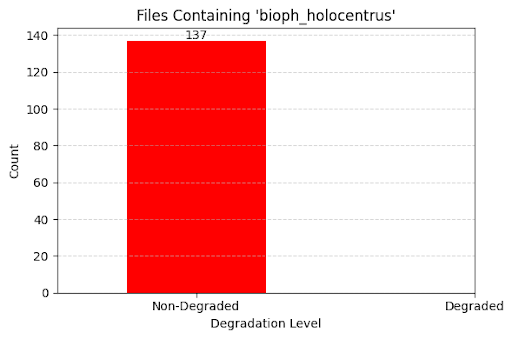
\includegraphics[height=1.0\textheight,width=1.0\textwidth,keepaspectratio]{images/knowledge_graph_results_4.png}
        \end{column}
    \end{columns}
\end{frame}

\begin{frame}{Knowledge Graphs - Future Work}
    \begin{itemize}
        \item Ensure future links are:
        \begin{itemize}
            \item Semantically cohesive (i.e. not predicting Dry Season $\rightarrow$ Degradation)
            \item Not a byproduct of a biased dataset
            \item Add more data (Costa Rica)
        \end{itemize}
        \item Ensure the graph is computational efficient
        \item Continue working on the binary classifier with Costa Rica data
        \item Work on knowledge graph visualization
    \end{itemize}
\end{frame}

\begin{frame}{Regression - Chi-Square Tests}
    \begin{figure}
        \centering
        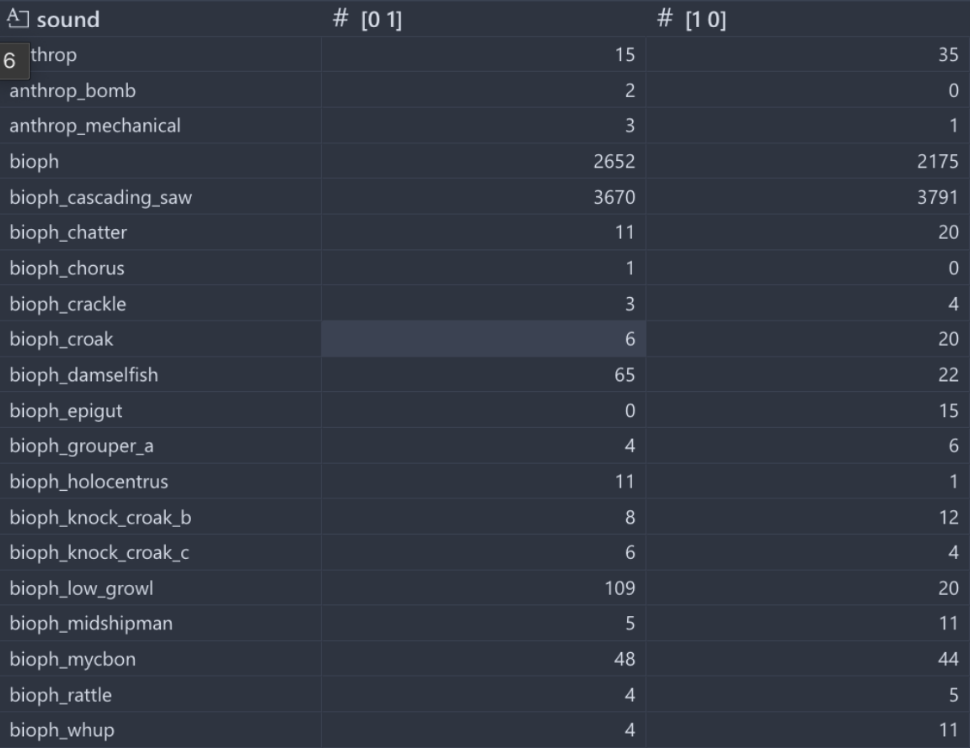
\includegraphics[height=0.8\textheight,width=0.8\textwidth,keepaspectratio]{images/reefset_classes.png}
        \caption{Occurrence of ReefSet classes in degraded and non-degraded reefs}
    \end{figure}
\end{frame}

\begin{frame}{Regression - Chi-Square Tests}
    \begin{figure}
        \centering
        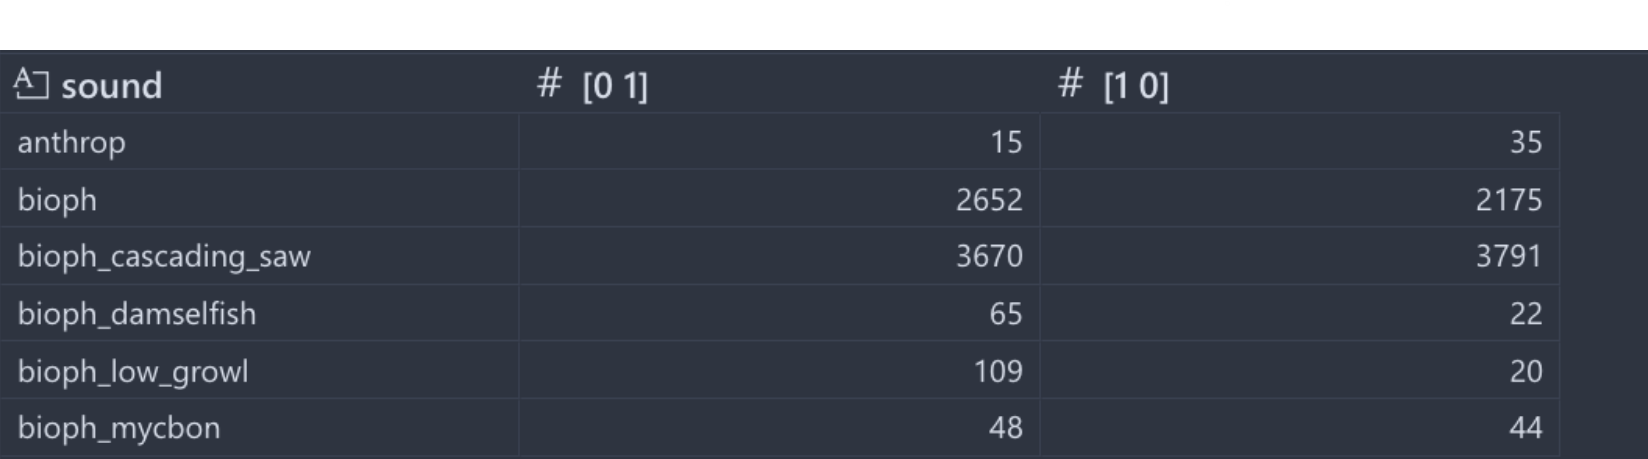
\includegraphics[height=0.8\textheight,width=0.8\textwidth,keepaspectratio]{images/chi_square_test.png}
        \caption{Classes with at least 30 occurrences in either degraded or non-degraded reefs}
    \end{figure}
    $\chi^2$: 523
    \newline
    P-value: $\sim$0
\end{frame}

\begin{frame}{Template Matching - Effectiveness}
    \begin{itemize}
        \item Able to find patterns but not the correct ones
            \begin{itemize}
                \item Domain shift, long/noisy xeno-canto templates cause issues
            \end{itemize}
    \end{itemize}
\end{frame}

\begin{frame}{Template Matching - Sound Separation}
    \begin{itemize}
        \item Exploring sound separation for better results
            \begin{itemize}
                \item Wisdom et al., 2020
            \end{itemize}
    \end{itemize}
    \begin{figure}
        \centering
        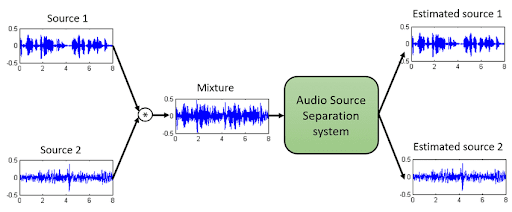
\includegraphics[height=0.7\textheight,width=0.7\textwidth,keepaspectratio]{images/sound_separation.png}
        \caption{Sound separation process (Duong, 2019)}
    \end{figure}
\end{frame}

\begin{frame}{Binary Classifier}
    \begin{columns}
        \begin{column}{0.5\textwidth}
            \begin{figure}
                \centering
                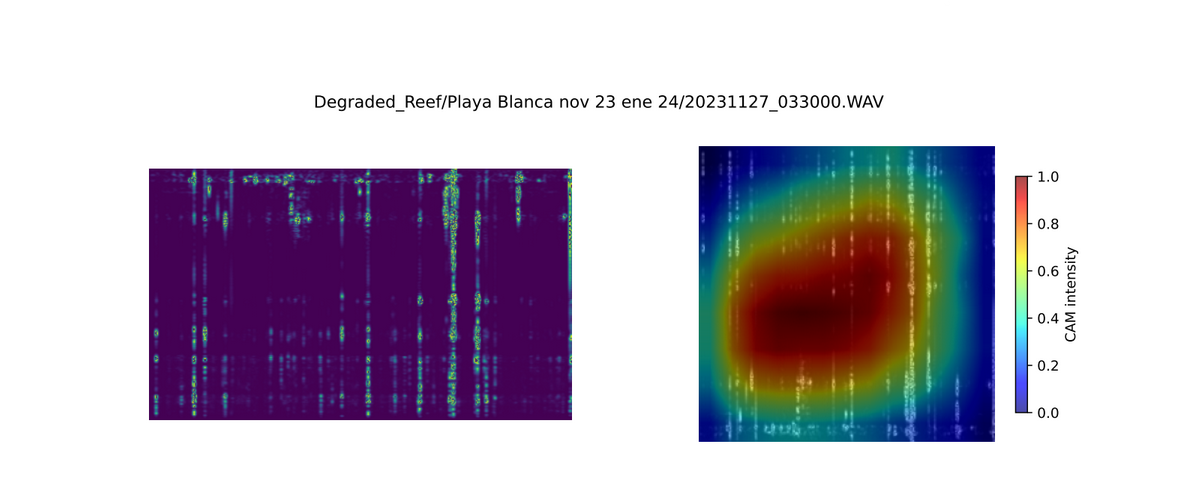
\includegraphics[height=0.75\textheight,width=0.75\textwidth,keepaspectratio]{images/degraded_gradcam.png}
                \caption{Degraded Grad-CAM}
            \end{figure}
        \end{column}
        \begin{column}{0.5\textwidth}
            \begin{figure}
                \centering
                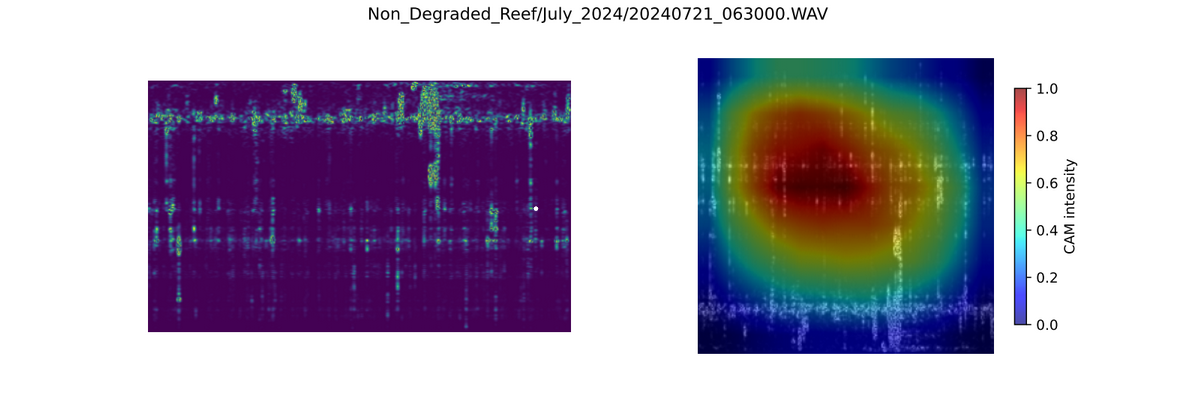
\includegraphics[height=0.75\textheight,width=0.75\textwidth,keepaspectratio]{images/non_degraded_gradcam.png}
                \caption{Non-degraded Grad-CAM}
            \end{figure}
        \end{column}
    \end{columns}
    \begin{figure}
        \centering
        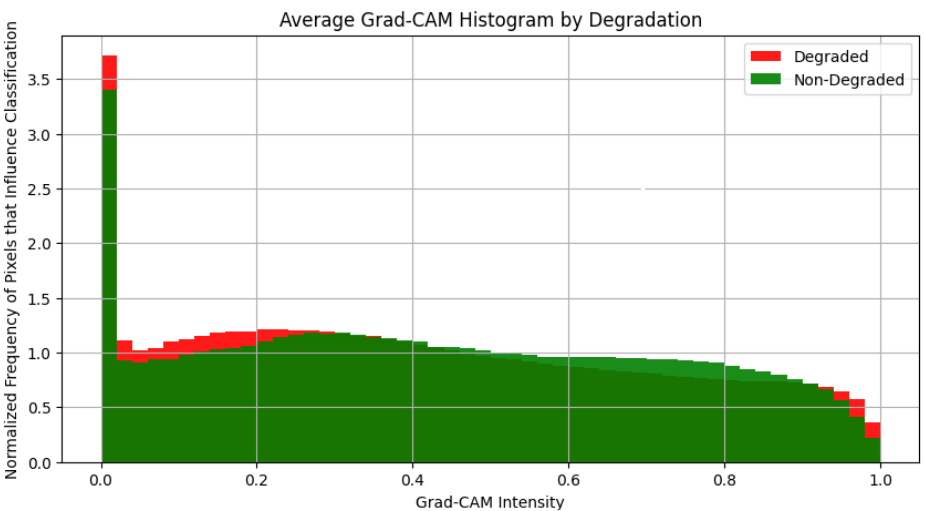
\includegraphics[height=0.5\textheight,width=0.5\textwidth,keepaspectratio]{images/gradcam_histogram.png}
        \caption{Grad-CAM histogram over 200 degraded and non-degraded samples}
    \end{figure}
\end{frame}

\begin{frame}{Binary Classifier}
    \begin{columns}
        \begin{column}{0.5\textwidth}
            \begin{figure}
                \centering
                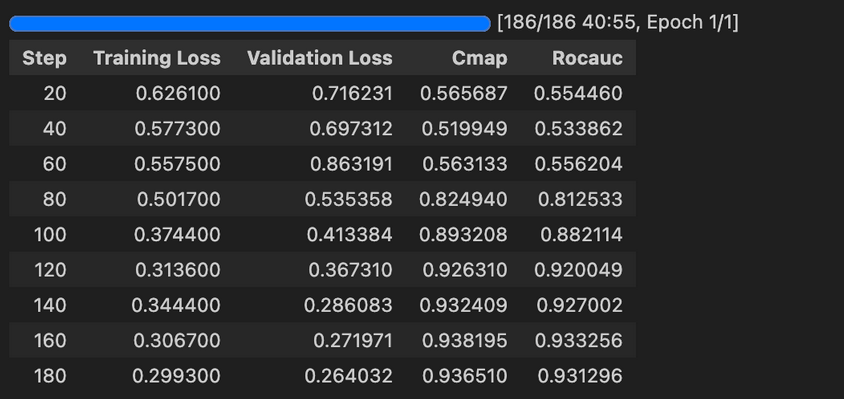
\includegraphics[height=1.0\textheight,width=1.0\textwidth,keepaspectratio]{images/binary_classifier_metrics_1.png}
                \caption{Binary classifier training metrics}
            \end{figure}
        \end{column}
        \begin{column}{0.5\textwidth}
            \begin{figure}
                \centering
                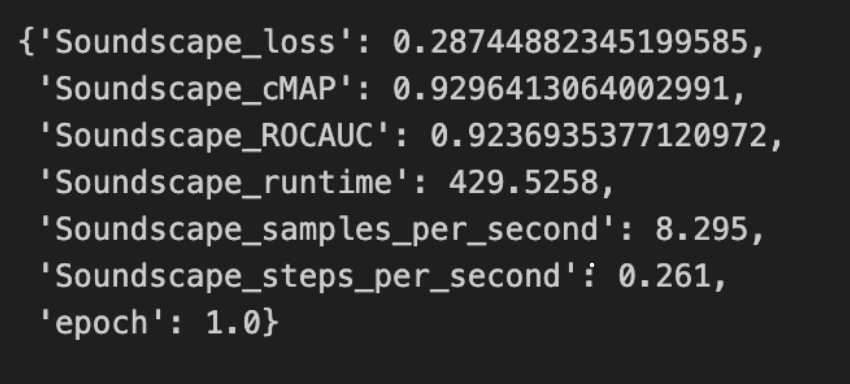
\includegraphics[height=1.0\textheight,width=1.0\textwidth,keepaspectratio]{images/binary_classifier_metrics_2.png}
                \caption{Final binary classifier metrics}
            \end{figure}
        \end{column}
    \end{columns}
\end{frame}

\begin{frame}{Site Separation}
    \begin{itemize}
        \item 
    \end{itemize}
\end{frame}

\begin{frame}{D3.JS Visualization}
    \begin{itemize}
        \item 
    \end{itemize}
\end{frame}